\documentclass[11pt]{article}
\usepackage{euscript}
\usepackage{amsmath}
\usepackage{amsthm}
\usepackage{amssymb}
\usepackage{epsfig}
\usepackage{xspace}
\usepackage{amsmath,amssymb,amsthm}
\usepackage{graphicx}
\usepackage[margin=1in]{geometry}
\usepackage{fancyhdr}
\usepackage{color}
\usepackage{url}
%%%%%%%%%%%%%%%%%%%%%%%%%%%%%%%%%
\setlength{\textheight}{9in}
\setlength{\topmargin}{-0.600in}
\setlength{\headheight}{0.2in}
\setlength{\headsep}{0.250in}
\setlength{\footskip}{0.5in}
\flushbottom
\setlength{\textwidth}{6.5in}
\setlength{\oddsidemargin}{0in}
\setlength{\evensidemargin}{0in}
\setlength{\columnsep}{2pc}
\setlength{\parindent}{1em}
\setlength{\parindent}{0pt}
\setlength{\parskip}{5pt plus 1pt}
\setlength{\headheight}{13.6pt}
%%%%%%%%%%%%%%%%%%%%%%%%%%%%%%%%%
\usepackage{epsfig}
\usepackage{xspace}
\usepackage{amsmath,amssymb,amsthm}
\usepackage{graphicx}
\usepackage[margin=1in]{geometry}
\usepackage{fancyhdr}
\usepackage{color}
\usepackage{url}
%%%%%%%  For drawing trees  %%%%%%%%%
\usepackage{tikz}
\usetikzlibrary{calc, shapes, backgrounds}
%%%%%%%%%%%%%%%%%%%%%%%%%%%%%%%%%
\setlength{\textheight}{9in}
\setlength{\topmargin}{-0.600in}
\setlength{\headheight}{0.2in}
\setlength{\headsep}{0.250in}
\setlength{\footskip}{0.5in}
\flushbottom
\setlength{\textwidth}{6.5in}
\setlength{\oddsidemargin}{0in}
\setlength{\evensidemargin}{0in}
\setlength{\columnsep}{2pc}
\setlength{\parindent}{1em}
\setlength{\parindent}{0pt}
\setlength{\parskip}{5pt plus 1pt}
\setlength{\headheight}{13.6pt}
%%%%%%%%%%%%%%%%%%%%%%%%%%%%%%%%%
\newcommand{\eps}{\varepsilon}
\renewcommand{\c}[1]{\ensuremath{\EuScript{#1}}}
\renewcommand{\b}[1]{\ensuremath{\mathbb{#1}}}
\renewcommand{\theenumi}{\alph{enumi}}
\newcommand{\s}[1]{\textsf{#1}}
\newcommand{\E}{\textbf{\textsf{E}}}
\renewcommand{\Pr}{\textbf{\textsf{Pr}}}
\newcommand\question[2]{\vspace{.25in}\hrule\textbf{#1: #2}\vspace{.5em}\hrule\vspace{.10in}}
\renewcommand\part[1]{\vspace{.10in}\textbf{(#1)}}
\newcommand\algorithm{\vspace{.10in}\textbf{Algorithm: }}
\newcommand\correctness{\vspace{.10in}\textbf{Correctness: }}
\newcommand\runtime{\vspace{.10in}\textbf{Running time: }}
\pagestyle{fancyplain}

\graphicspath{ {.} }

\lhead{\textbf{\NAME\ (\UNI)}}
\chead{\textbf{HW\HWNUM}}
\rhead{COMS W4721, \today}


\newcommand\NAME{Daniel Kronovet}  
\newcommand\UNI{003349897}    
\newcommand\HWNUM{01}          

\begin{document}

%%%%%%%%%%%%%%%%%%%%%%%%%%%%%%%%%%%%%%%%%%%%%%%%%%%%
%%%%%%%%%%%%%%%%%%%%%%%%%%%%%%%%%%%%%%%%%%%%%%%%%%%%
%%%%%%%%%%%%%%%%%%%%%%%%%%%%%%%%%%%%%%%%%%%%%%%%%%%%

\section*{Problem 1 (maximum likelihood)}

Part 1:
\begin{enumerate}
\item What is the joint likelihood of the data $(x1,...,xN)$?

Assuming $x_i$ are all drawn iid, the joint likelihood is the product of the individual probabilities of all $x_i$:

\[
L_{\pi} = \prod_{i=1}^{n} \pi^{x_i}(1-\pi)^{1-x_i}
\]

\item Derive the maximum likelihood estimate $\hat \pi_{ML}$ for $\pi$.

\[
ln L_{\pi} = \sum_{i=1}^{n} x_i ln(\pi) + (1-x_{i}) ln(1-\pi)
\]
\[
ln L\prime_{\pi} = \sum_{i=1}^{n} \frac{x_i}{\pi} + \frac{1 - x_i}{1-\pi}(-1) = 0
\]
\[
 \frac{\sum x_i}{\pi} = \frac{\sum 1 - x_i}{1-\pi}
\]
\[
 \frac{\sum x_i}{\pi} = \frac{n - \sum x_i}{1-\pi}
\]
\[
\sum x_i - \pi \sum x_i  = n\pi - \pi \sum x_i
\]
\[
\sum x_i  = n\pi
\]
\[
\frac{\sum x_i}{n}  = \hat \pi_{ML}
\]

\item Explain why this maximum likelihood estimate makes intuitive sense.

For this distribution, the Maximum Likelihood estimator is the sum of all data points (in effect, the number of successes), divided by the total number of trials -- giving the proportion of successes. This makes tremendous sense as the MLE, as $\pi$ is meant to represent the likelihood of success of any given trial.

\end{enumerate}

Part 2:
\begin{enumerate}
\item What is the joint likelihood of the data $(x1,...,xN)$?

\[
L_{\lambda} = \prod_{i=1}^{n} \frac{\lambda^{x_i}}{x!} e^{-\lambda}
\]

\item Derive the maximum likelihood estimate $\hat \lambda_{ML}$ for $\lambda$.

\[
ln L_{\lambda} = \sum_{i=1}^{n} x_i ln(\lambda) - ln(x!) - \lambda
\]
\[
ln L\prime_{\lambda} = \sum_{i=1}^{n} \frac{x_i}{\lambda} - 1 = 0
\]
\[
\frac{\sum x_i}{\lambda} = n
\]
\[
\frac{\sum x_i}{n} = \hat \lambda_{ML}
\]

\item Explain why this maximum likelihood estimate makes intuitive sense.

Similarly to Part 1, the parameter $\lambda$ of a poisson distribution is meant to represent the average rate of occurrence of the phenomenon being modeled. As such, the MLE of the parameter would be the average of all the values in the sample.

\end{enumerate}



\section*{Problem 2 (Bayes rule)}

\begin{enumerate}
\item Use Bayes rule to derive the posterior distribution of $\lambda$ and identify the name of this distribution.

By Bayes rule, we know that:
\[
P(\lambda | x) = \frac{P(x | \lambda) P(\lambda)}{P(x)}
\]

Given that we are interested in $\lambda$, we can discard the denominator (which ultimately does not involve $\lambda$) and rewrite this equation as:

\[
P(\lambda | x) \propto P(x | \lambda) P(\lambda)
\]

We can then expand the right side of the equation into the joint distribution of $P(x, \lambda)$:

\[
P(\lambda | x) \propto  (\prod_{i=1}^{n} \frac{\lambda^{x_i}}{x!} e^{-\lambda}) \frac{\beta_1^{\alpha_1}}{\Gamma(\alpha_1)} \lambda^{\alpha_1 - 1} e^{-\beta_1 \lambda}
\]
\[
\propto  (\frac{\lambda^{\sum x_i}}{\prod x!} e^{-n\lambda}) \frac{\beta_1^{\alpha_1}}{\Gamma(\alpha_1)} \lambda^{\alpha_1 - 1} e^{-\beta_1 \lambda}
\]
\[
\propto  \frac{\beta_1^{\alpha_1}}{\Gamma(\alpha_1) \prod x!} \lambda^{(\sum x_i + \alpha_1) - 1} e^{-\lambda (n + \beta_1)})
\]

From this we have enough to learn the parameters of the posterior Gamma distribution: $\alpha_2 = \sum x_i + \alpha_1$ and $\beta_2 = n + \beta_1$. This result is still not the complete distribution, however: the fraction is not in the correct form for a Gamma, nor have we addressed the denominator which we dropped earlier. We know, however, that the final distribution must integrate to 1, which allows us to derive the correct values for the other terms (although we will not do so here).

\item What is the mean and variance of $\lambda$ under this posterior? Discuss how this relates to your solution to Part 2 of Problem 1.

The posterior $\lambda$ is $~Gamma(\sum x_i + \alpha_1, n + \beta_1)$

As such, the mean of $\lambda = \frac{\alpha_2}{\beta_2} = \frac{\sum x_i + \alpha_1}{n + \beta_1}$.

The variance is $\frac{\alpha_2}{\beta_2^2} = \frac{\sum x_i + \alpha_1}{(n + \beta_1)^2}$.

In 1.2, we saw that: $\frac{\sum x_i}{n} = \hat \lambda_{ML}$.

There is a clear parallel to the Bayesian posterior mean: $\frac{\sum x_i + \alpha_1}{n + \beta_1} = E(\lambda)$, with the difference being the influence of the prior parameters $\alpha_1$ and $\beta_1$. This relationship represents the Bayesian insight by which our posterior distribution is determined by an interaction between our prior beliefs ($\alpha_1, \beta_1$) and our data ($\sum x_i, n$).

\end{enumerate}



\section*{Problem 3 (Linear regression)}

Part 1
\begin{enumerate}
\item Print the numbers you obtain for the vector $\hat w_{ML}$. Using the labels of each dimension contained in the readme file, explain what the sign of each value in $\hat w_{ML}$ says about the relationship of the inputs to the output.

\begin{table}[!th]
\centering
\begin{tabular}{|l|r|}
\hline
Dimension & Weight \\
\hline
Intercept & 23.42352482 \\
Num Cylinders & -0.5759929  \\
Displacement & 0.90318199 \\
Horsepower & -0.12294213 \\
Weight & -5.78808517 \\
Acceleration & 0.21887044 \\
Model Year & 2.77543049 \\
\hline
\end{tabular}
\caption{$\hat w_{ML}$}
\label{ex:table}
\end{table}

First, we note that when all dimensions are at their (centered) average, the intercept (average) for MPG is ~23.42. Beyond that, the dimensions of Displacement, Acceleration, and Model Year are positively correlated with MPG, while Num Cylinders, Horsepower, and Weight, are negatively correlated.

Of these, we see that Weight is the most strongly negatively correlated with MPG, which is sensible as increased weight directly translates into increased energy necessary to move the car, reducing MPG. Interestingly, Model Year has by far the strongest positive correlation with MPG, suggesting that secular fuel efficiency improvements year over year play a bigger role in improving MPG than any other single factor. 

\item Use the least squares solution to predict the outputs for each of the 20 testing examples. Repeat this process of randomly splitting into training and testing sets 1000 times. Each time, calculate the mean absolute error of the resulting predictions, MAE = $\frac{1}{20} \sum_{i=1}^{20} \mid y_{test} - y_{pred} \mid$. What is the mean and standard deviation of the MAE for these 1000 tests?

After running 1000 iterations, $\mu_{MAE} = 2.71242956285$, while $\sigma_{MAE} = 0.49817244422$

\end{enumerate}

Part 2
\begin{enumerate}
\item In a table, print the mean and standard deviation of the RMSE as a function of $p$. Using these numbers argue for which value of $p$ is the best.

As this table shows, setting $p$ = 3 gives both the lowest RMSE and the lowest variance for any value of $p$.

\begin{table}[!th]
\centering
\begin{tabular}{|l|c|r|}
\hline
$p$ & Mean & Std \\
\hline
1 & 3.44030468834 & 0.672995051589 \\
2 & 2.75919186824 & 0.623061482354 \\
3 & 2.64085582004 & 0.602524538829 \\
4 & 2.73039848277 & 0.697498334382 \\
\hline
\end{tabular}
\caption{RMSE by $p$}
\label{ex:table}
\end{table}

\item For each value of $p$, collect $y_{test} - y_{pred}$ for each test example. (Observe that this number can be negative, and there are 20 x 1000 in total.) Plot a histogram of these errors for each $p$.

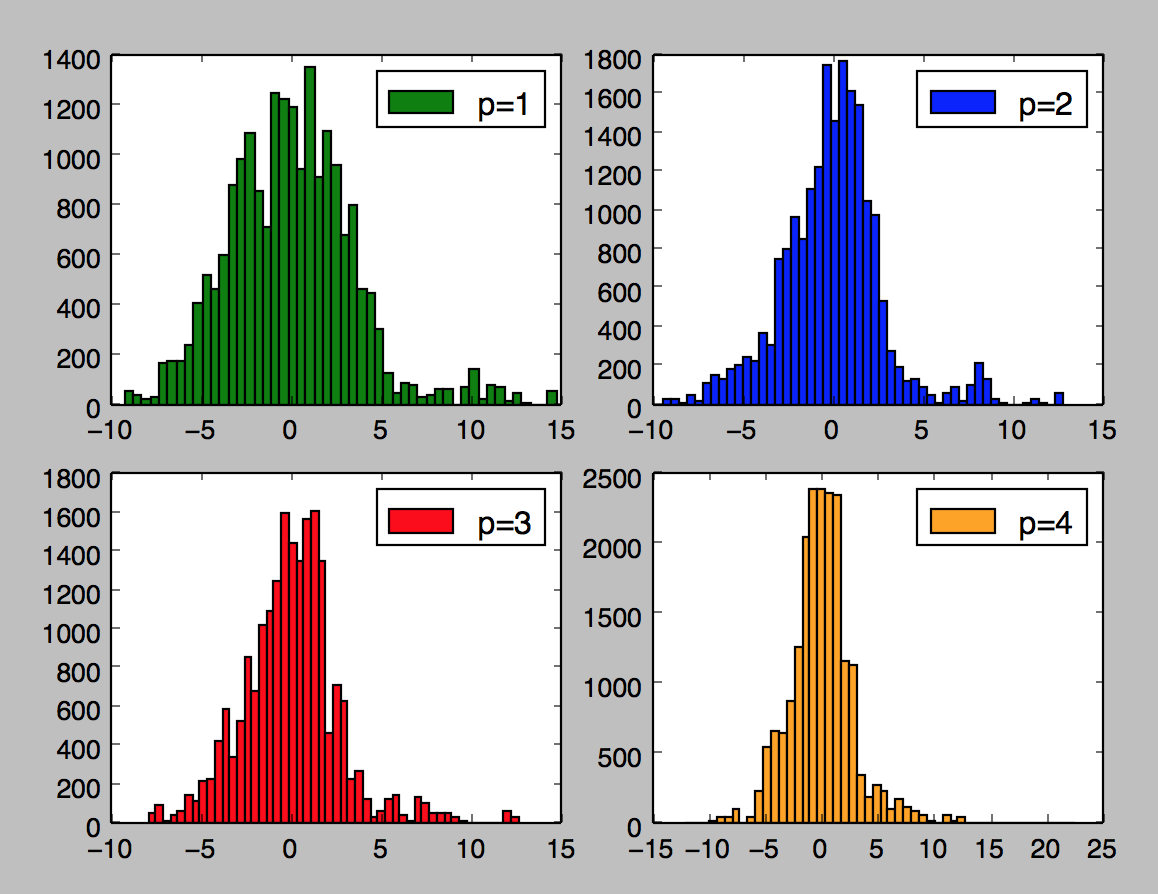
\includegraphics[scale=0.8]{errors_hist.png}


\item For each $p$, use maximum likelihood to fit a univariate Gaussian to the 20,000 errors from Part 2(b). Describe how you calculated the maximum likelihood values for the mean and variance (this is a univariate case of what we did in class, so no need to re-derive it). What is the log likelihood of these empirical errors using the maximum likelihood values for the mean and variance? Show this as a function of $p$ and discuss how this agrees/disagrees with your conclusion in Part 2(a). What assumptions are best satisfied by the optimal value of $p$ using this approach?

To fit the Gaussian, we calculated both $\hat \mu_{ML}$ and $\hat \sigma^2_{ML}$ using the standard maximum-likelihood estimators for these parameters: $\frac{1}{n} \sum_{i=1}^{n} x_i$ and $\frac{1}{n-1} \sum_{i=1}^{n} (x_i - \hat \mu_{ML})^2$.

Looking at this table, $p = 3$ again appears to create the strongest model. The variance (although not the mean) of the error is lowest with this model. Additionally, the log likelihood of this error is the greatest, although by a small margin, compared to all other models. This supports our conclusions in 2(a), where we identified $p = 3$ as being the strongest model.

\begin{table}[!th]
\centering
\begin{tabular}{| l| c | c | r|}
\hline
$p$ & Mean & Var & Log Likelihood \\
\hline
1 & 0.0163194355852 & 3.50549766331 & -53464.9206058 \\
2 & -0.0285981551706 & 2.82852246649 & -49173.3602374 \\
3 & 0.0409854631276 & 2.70840898169 & -48305.4980812 \\
4 & 0.0593496182852 & 2.81743994052 & -49094.8436665 \\
\hline
\end{tabular}
\caption{Log Likelihood of error by $p$}
\label{ex:table}
\end{table}

\end{enumerate}


\end{document}
